\section{Jenkins}
\label{sec:jenkins}
    Jenkins byl dřív známý jako Hudson a přejmenoval se po neshodě s~Oracle~\cite{jenkins-hudson}. Oba projekty pak nějakou dobu byly udržovány souběžně. Oracle svůj systém Hudson oficiálně nikdy nepřestal vyvíjet, ale poslední vydání je ze začátku roku 2016. V~následujícím textu se budu věnovat pouze Jenkins, který je dodnes aktivně udržován a má velkou komunitu.

    Hlavní výsadou Jenkins oproti ostatním \CICD systémům je rozšiřitelnost pomocí pluginů.
    %\todo{popsat ze jenkins je jenom o pluginech}\blind[1]

    Architektura Jenkins je master+agents~\cite{jenkins-architecture}. Stavová master instance poskytuje \glstext{API} a webové \glstext{GUI} a koordinuje práci jednotlivých bezstavových agentů (workerů). Je zajímavé, že Jenkins nevyužívá tradiční relační databázi, ale persistuje data přímo na disk v~formátu \glstext{XML}.

    \subsection{Instalace a konfigurace}
        Instalace Jenkins z~oficiálního balíčku je přímočařá. Nejprve jsem zaregistroval Jenkins \glstext{APT} repozitář \code{pkg.jenkins.io} a aplikaci nainstaloval. Jenkins ale odmítal nastartovat, protože mu chyběl Java runtime. Očekával bych, že aplikační balíček bude mít nezbytné závislosti minimálně v~\textit{suggested packages}. Jenkins v~aktuální verzi podporuje pouze Java 8~\cite{jenkins-java}. To je \glstext{LTS} verze z~března 2014, která má komerční podporu pouze do ledna 2019~\cite{oracle-eol}.

        Při prvním zobrazení webového rozhraní se provádí konfigurace a volitelná instalace rozšíření. Na rozdíl od např. GitLabu nebo Wordpressu vyžaduje Jenkins výchozí administrátorské heslo, které vygeneroval na disk.

        V~roce 2018 přišel Jenkins s~možností nahradit ruční klikání konfigurace ve webovém rozhraní kódem (\glstext{CasC})~\cite{jenkins-casc}. Některá klíčová nastavení, konkrétně třeba správa rozšíření, je zatím nestabilní. Dále je nahlášena celá řada nekompatibilit s~různými rozšířeními \code{jenkins-casc-compat}.

        \begin{iffigure}
            \centering
                \begin{minted}[frame=lines,framesep=2mm,linenos]{python}
pipeline {
    agent none
    stages {
        stage('Jekyll Build') {
            agent {
                docker 'composer:1.8'
            }
            steps {
                checkout scm
                sh 'make build'
            }
        }
        stage('Deploy') {
            agent {
                docker 'ditemikuthesisdemo/deploy:1.0'
            }
            steps {
                sh 'make deploy'
            }
        }
    }
}
                \end{minted}
            \caption{Ukázka definice deklarativní pipeline v \code{Jenkinsfile}. Pro správu závislostí se využívají se předpřipravané Docker obrazy. V prvním kroku se používá oficiální univerzální obraz, v kroku s nasazením je obraz vytvořený pro tento projekt.}
        \end{iffigure}


        Každý projekt je na Jenkins nutné založit a nakonfigurovat ručně. Některá rozšíření tento problém řeší, například \code{GitHub Branch Source Plugin}~\cite{jenkins-plugins-gbs} sleduje všechny repozitáře vybraných GitLab uživatelů a pokud v~nich najde \code{Jenkinsfile}, založí pro repozitář nový projekt na Jenkins. Původně byly Jenkins projekty konfigurovatelné jenom z~webového rozhraní a \glstext{API}. V~roce 2014 byla publikován \code{Pipeline Plugin}, který umožňuje popsat konfiguraci projektu skriptem. Na to v~roce 2016 navázalo rozšíření \code{Pipeline Model Definition Plugin}, které přináší podporu pro deklarativní popis pipeline, kde Jenkins říkáme co se má stát, ale ne nutně \textit{jak}. Deklarativní pipeline je doporučený způsob nastavení Jenkins projektů~\cite{jenkins-best-practices}.

        Problém Jenkins je uživatelské rozhraní. Ve výchozím stavu má \glstext{UI} celou řadu velmi problematických částí: několika-úrovňové menu, které vyžaduje přesný pohyb myší; nesjednocené symboly, navíc často nekonvenční (například modrá koule u~úspěšného jobu místo klasické zelené); konfigurace a všechny formuláře jsou složité a běžně obsahují 100+ vstupů. Rozšíření Blue Ocean nabízí alternativní \glstext{UI} pro zobrazení průběhu a výsledků buildů~\cite{jenkins-plugin-blueocean}. Pokud uživatelé konfigurují projekty výhradně přes \code{Jenkinsfile}, nemusí do původního rozhraní vůbec přistupovat. Osobně mi rozhraní přišlo hezké, ale oproti konkurenčním \CICD pomalé.

    \subsection{Rozšiřitelnost}
        Jenkins má v~oficiálním registru přes $1\,500$ rozšíření. Používaných je jich ale jenom zlomek; jak ukazuji \pfxref{na grafu}{fig:jenkins-plugins} často instalovaných rozšíření je jenom kolem $200$. Velmi překvapivé bylo zjištění, že rozšíření jsou často aktualizovaná. \pfxref{Z~grafu}{fig:jenkins-plugins-update} lze vidět, že přes $600$ rozšíření mělo vydání v~posledním roce.

        \afterpage{
            \begin{iffigure}
                \centering
                \begin{subfigure}[b]{\textwidth}
                    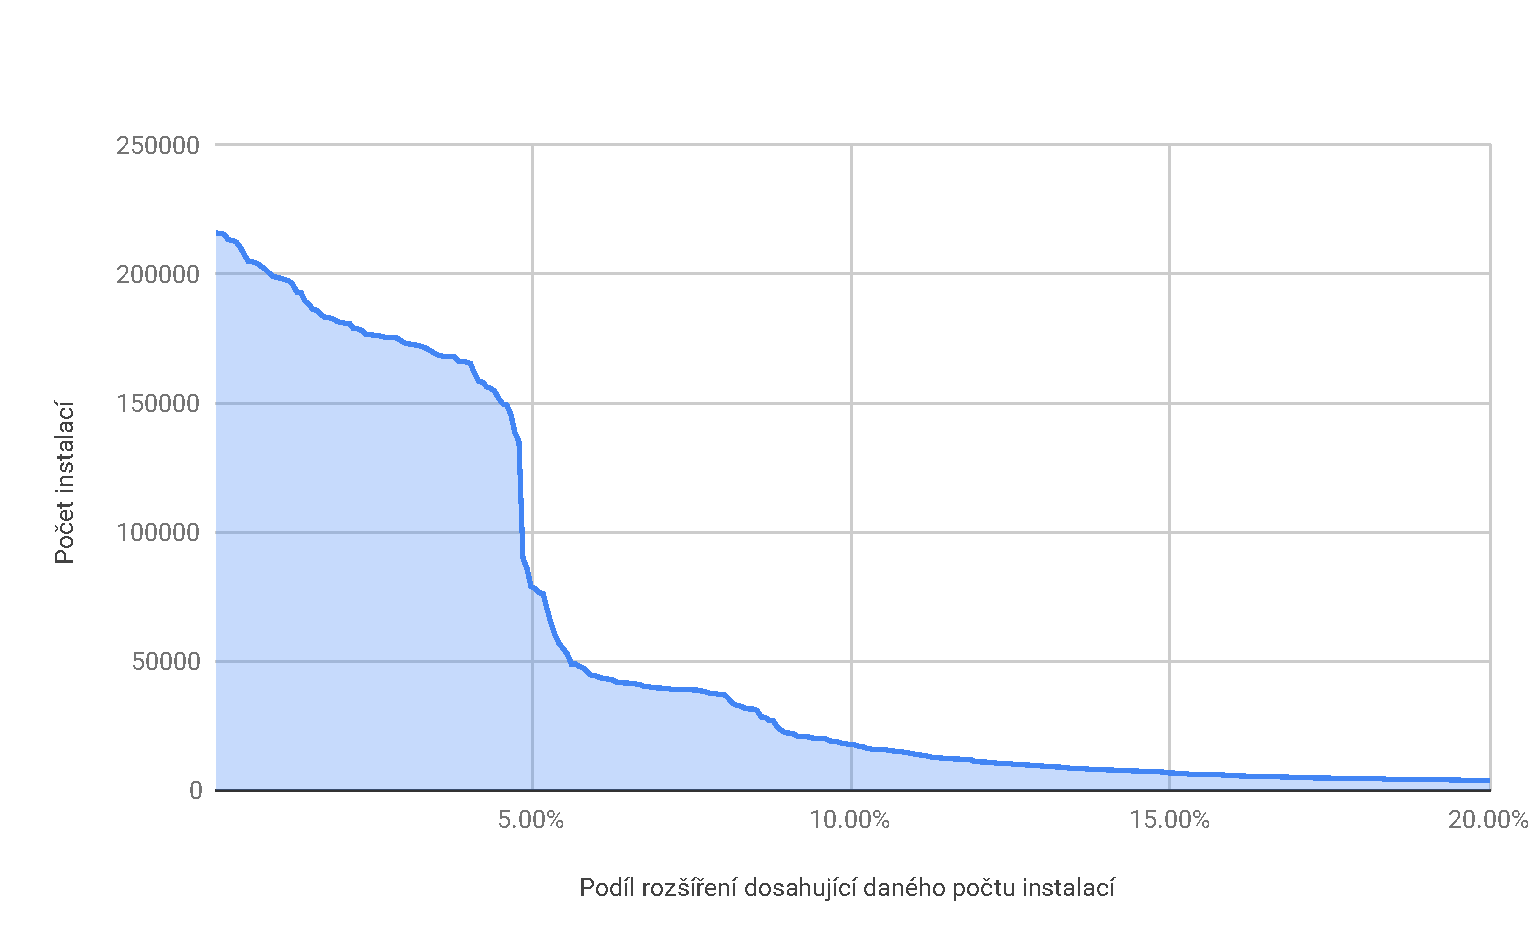
\includegraphics[width=\textwidth,height=9cm,keepaspectratio]{media/jenkins-plugins.pdf}
                    \caption{Rozdělení počtu instalací. Oříznutých 80~\% je klesající dlouhý ocas. Pouze zhruba $80$ rozšíření má víc instalací než $100\,000$. To jsou pluginy, které se nabízí administrátorům při první konfiguraci Jenkins. Necelých $200$ rozšíření má víc než $10\,000$ instalací. Přes 60~\% publikovaných rozšíření má méně než $1\,000$ instalací.}
                    \label{fig:jenkins-plugins}
                \end{subfigure}

                \begin{subfigure}[b]{\textwidth}
                    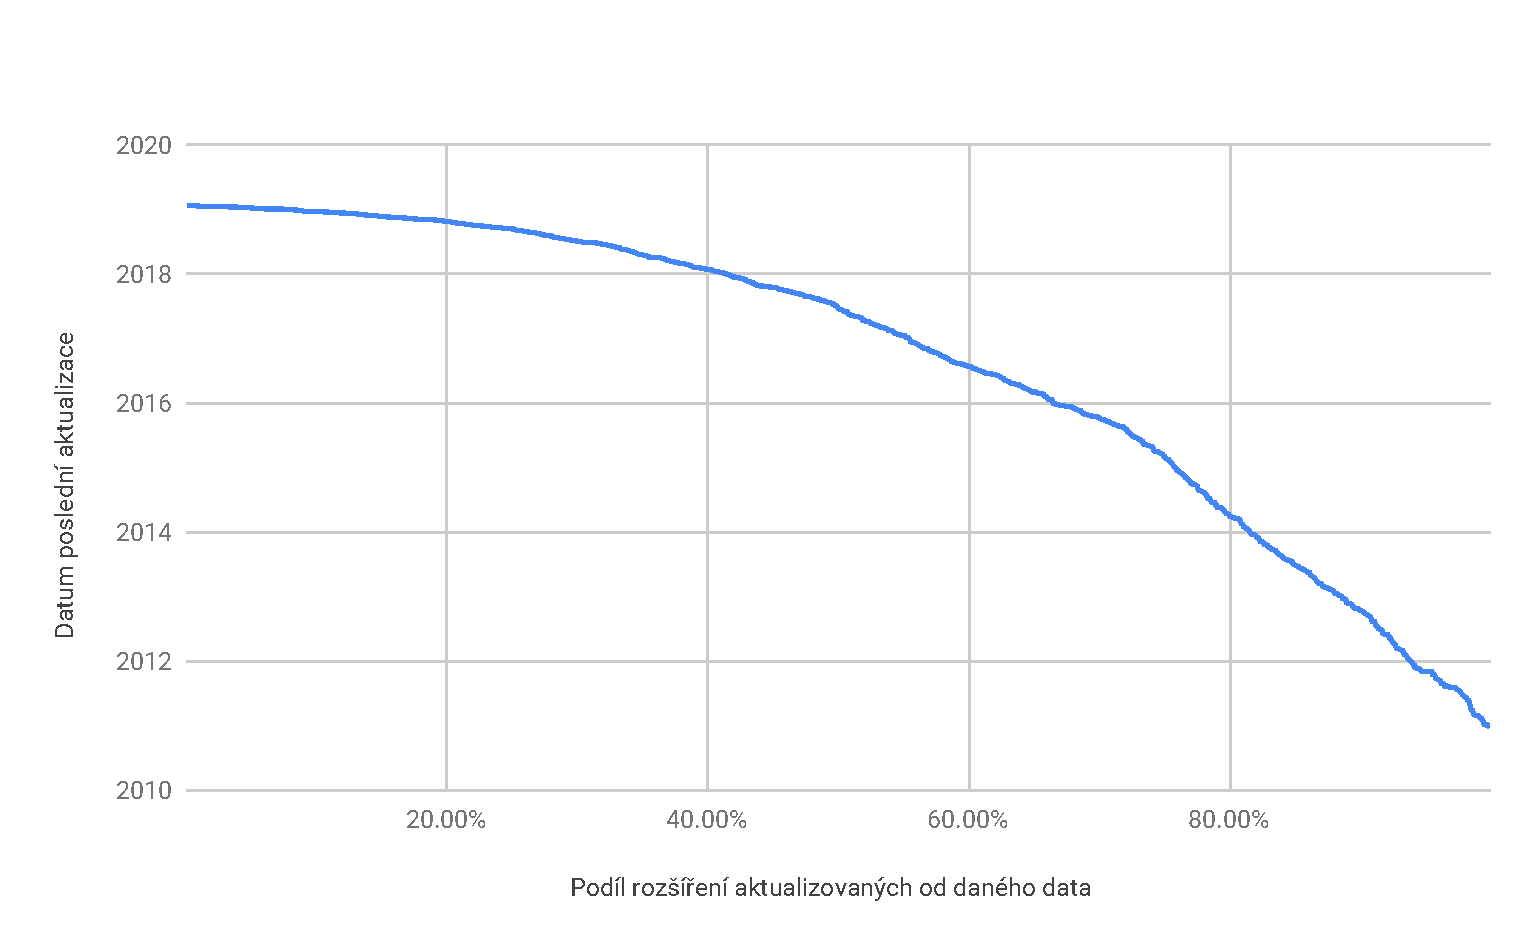
\includegraphics[width=\textwidth,height=9cm,keepaspectratio]{media/jenkins-plugins-update.pdf}
                    \caption{Rozdělení podle poslední aktualizace. Skoro 30~\% byla aktualizována v~posledním půl roce. 40~\% rozšíření mělo alespoň jednu aktualizaci za poslední rok.}
                    \label{fig:jenkins-plugins-update}
                \end{subfigure}

                \caption{Zdroj: data vytažena z~\url{https://plugins.jenkins.io/}, agregace a vizualizace vlastní. Data jsou dostupná na přiloženém mediu v~\code{appendix/jenkins-plugin-*.csv}.}
            \end{iffigure}
            \clearpage
        }

        Celkově působí Jenkins velmi roztříštěně. Některá rozšíření mají dokumentaci na Jenkins Wiki, jiné na portálu Jenkins Plugins a zbytek na vlastních dedikovaných stránkách nebo na GitHubu. Část pluginů má nějaký obsah na všech těchto místech a dohledat konkrétní informace bývá obtížné. Velký problém je poznat, jaká rozšíření nainstalovat. Pipelines jsou pro moderní použití Jenkins nezbytné, ale administrátor to musí sám vyčíst z~blogů a odkoukat od ostatních. Je na trhu prostor pro svéhlavou distribuci Jenkins, která by obsahovala \textit{best-practice} rozšíření a konfiguraci.

        Jenkins umožňuje upravit prakticky cokoliv. Na rozdíl od GitLabu, kde vývojář může konfigurovat pipeline a spouštět libovolné procesy, na Jenkins lze upravit samotné rozhraní. Šlo by například rozšířit Jenkins o~stránku s~přehledem nasazených prostředí, podobně jako má GitLab své Environments. Je pak ale na zvážení, jestli není praktičtější podobně velké úpravy vyčlenit do samostatné webové aplikace.

        Kromě toho existují rozšíření, které umožňují spouštět skripty v~rámci jobů. Například \textit{Pipeline: Groovy} načte zdrojový kód umožňuje ho v~jobu spustit. To bývá užitečné pro vyčlenění společné funkcionality napříč několika projekty a pro zpřehlednění pipeline.

    \subsection{Zabezpečení}
        Stejným způsobem kterým Jenkins deleguje funkcionalitu na pluginy, přenáší zodpovědnost i za bezpečnost. Jádro Jenkins mělo za rok 2018 nahlášeno 53 \glstext{CVE}, rozšíření pro Jenkins skoro 100~\cite{cve-jenkins}. Čím víc rozšíření je do Jenkins nainstalováno, tím větší je plocha pro potenciální útočníky. Izolace klientů o~něco horší než u~GitLabu. Přestože oba systémy podporují různé úrovně izolace samotných jobů, nastavení práv pro webovou administraci Jenkins je velmi složité a nepřehledné. Tak jako všechno ostatní deleguje Jenkins i \glstext{ACL} na rozšíření. Základní rozšíření \textit{Matrix-based security} umožňuje nastavit každému uživateli nebo skupině práva k~nějaké akci. Jenom u~zdroje \textit{Job} je ale 9 oprávnění a není dobře zdokumentované, co přesně umožňují.

        Některé integrace, například GitHub, podle dokumentace umožňují dynamicky přiřazovat práva podle uživatelů přiřazených k~danému repozitáři. Tuto funkci se mi ale nepodařilo zprovoznit; buď byl projekt úplně veřejný, nebo úplně nedostupný.

        Izolace v~rámci samotných agentů/workerů může být perfektní. Je dokonce i možné dynamicky reagovat na využití a zapínat a vypínat agenty v~cloudu. Některá rozšíření umožňují využívat i krátkožijící virtuální stroje v~cloudu jako je \glstext{AWS} CodeBuild~\cite{jenkins-codebuild} nebo \glstext{GCP} Cloud Build.

        \begin{iffigure}
            \centering
            \makebox[\textwidth][c]{
                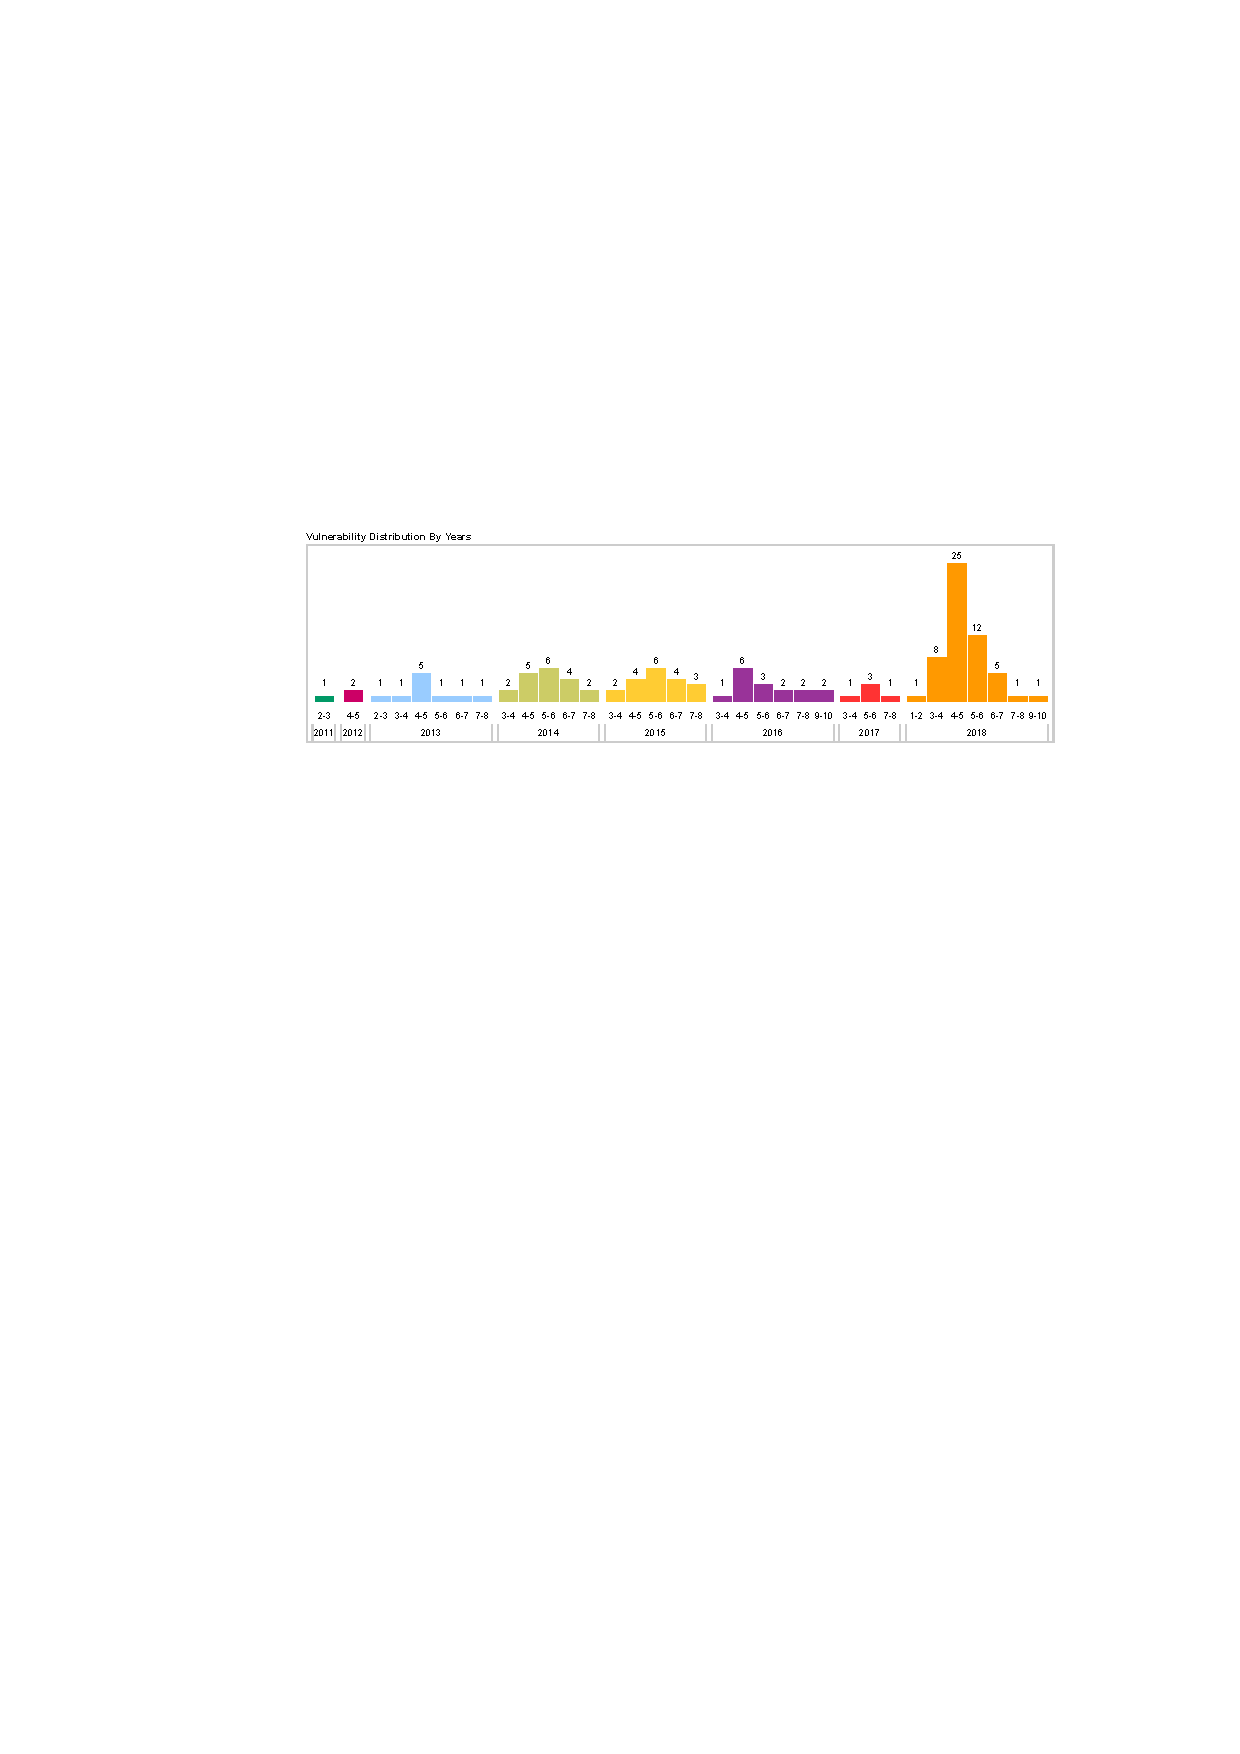
\includegraphics[width=1.2\textwidth]{media/jenkins-cve.pdf}
            }
            \caption{Rozložení Jenkins \glstext{CVE} a přiřazené skóre podle \glstext{CVSS}. Většina nahlášených bezpečnostních chyb bylo \glstext{XSS} a únik informací. Nejvážnější problém v~jádru v~roce 2018 byla možnost neomezeného spouštění procesů na masteru, které mohl využít každý uživatel s~právem přidat nový agent~\cite{cve-jenkins}.}
            \label{fig:gitlab-review-cycle}
        \end{iffigure}

    \subsection{Dostupnost}
        Tím že Jenkins je výhradně ke spouštění jobů, dostupnost neřeší. Myšlenka je taková, že Jenkins periodicky skenuje různé repozitáře a při detekci změny začne nový job. V~případě výpadku se pouze job zpozdí. Na rozdíl od GitLabu neposkytuje další vývojářům další funkce jako je repozitář verzovacího systému, správa úkolů a podobně. Přesto je výpadek Jenkins problematický i při každodenním užívání: projekty nemůžou využívat spouštění jobů z~\glstext{API} a vývojáři nemůžou zobrazovat logy a využívat artifacts.

        Při instalaci ale i při aktualizaci rozšíření vyžaduje Jenkins restart. Některá rozšíření lze nainstalovat i bez restartu, ale pro upgrade je vyžadován~\cite{jenkins-norestart}. Nabízí možnost restartovat po dokončení všech právě běžících jobů, nebo manuální restart. V~mém testovacím prostředí trvá restart přes 30 vteřin. Stejně tak je nutný restart při upgrade celého jádra.

        Jenkins je stavová aplikace persistující na disk. Není možné spustit víc replik a sdílet úložiště například přes \glstext{NFS}, protože Jenkins drží část informací jenom v~paměti. Nejlepší dostupnosti lze dosáhnout použitím failoveru (\textit{cold standby}). Je nutné zajistit, aby aktivní proces byl nejprve ukončen a persistoval všechny stavy na disk a až poté je možné zapnout standby instanci~\cite{jenkins-ha}. Ve výsledku tedy čekáme na vypnutí a zapnutí celé aplikace a doba výpadku je stejně dlouhá jako bez použití failoveru, ale infrastruktura pak není závislá na dostupnosti jednoho datacentra. Stojí za povšimnutí, že tuto formu failoveru získáme bez práce při použití libovolného orchestrátoru kontejnerů (Docker Swarm, Kubernetes, OpenShift, \ldots).

        Pokud se Jenkins restartuje, běžící joby se ztratí. V~administraci a v~\glstext{API} je možnost \textit{safe restart}, která pozastaví frontu jobů, nechá už běžící joby doběhnout a poté systém restartuje.

        Jelikož Jenkins nevyužívá databázi a všechna data persistuje na disk, je dostačují pravidelně vytvářet snapshot souborového systému (typicky dat v~\code{/var/lib/jenkins}).

    \subsection{Integrace}
        Jenkins lze používat s~libovolným externím repozitářem (GitHub/GitLab/Bitbucket/\ldots) a pomocí vhodného rozšíření lze na danou službu i posílat oznámení o~stavu. Jako jediný z~porovnávaných systémů dokonce podporuje i jiné verzovací systémy (Mercurial, SVN, \ldots) a dokonce je možné vytvořit pipeline která není na žádný repozitář vázaná.

        Nasazení na cílové servery je mimo kompetenci Jenkins. Existují rozšíření, která přidávají Groovy funkce použitelné v~Jenkins Pipeline, ale v~porovnání s~GitLab Jenkins nijak \CD nepodporuje (v~tom smyslu, že pokrývá pouze \CI).

    \subsection{Praktické nasazení projektů}
        \subsubsection{Projekt 1}
            Pro statický projekt jsem připravil pipeline využívající Docker. Kompilace Jekyll zdrojů potřebuje hodně závislostí a je nepraktické je instalovat přímo na hostitelské servery. To jsem otestoval \pfxref{v~sekci o~GitLab}{subsec:gitlab-p1}. V~Jenkins jsem ručně založil novou Pipeline a v~nastavení jsem vybral možnost \textit{Pipeline Script from \glstext{SCM}} -- to umožňuje verzovat Jenkinsfile přímo v~projektu. Alternativa je ručně psát pipeline přímo ve webové administraci Jenkins, což odporuje \textit{Infrastructure as Code}. Dále jsem musel ručně zadat cestu k~repozitáři. Narazil jsem na chybu v~Jenkins, která znemožňuje v~Pipeline klonovat lokální Git repozitáře. Tento problém jsem obešel uvedením vzdáleného repozitáře na GitLabu.

            Samotná deklarativní pipeline není složitá. Uvedl jsem docker obraz, ve kterém se má kompilace provést. Dále jsem rozdělil práci na dvě stages: build a deploy. Stejně jako GitLab umí Jenkins opakovat jednu stage bez nutnosti spouštět znovu celou pipeline, což se hodí pro přechodné chyby, pro deploy, rollback a podobně. V~samotných stages se pak spouští předpřipravené scripty, které využívám pro všechna testovaná \CICD prostředí.

        \subsubsection{Projekt 2}
            Pro toto nasazení jsem rozdělil Jenkins Pipeline na samostatné kontejnery: ke každé stage je přiřazen odlišný Docker Agent, který používá přesně daný image. Tím jsou zamknuty externí závislosti, jednotlivé projekty se navzájem neovlivňují a není potřeba žádné knihovny a podpůrný software předinstalovávat na testovací server.

            Při použití vlastních Docker obrazů pro build je vhodné, aby se vystavovaly v~\CI. V~případě sdílení daného obrazu mezi více projekty může být úplně vyčleněn do samostatné pipeline.

        \subsubsection{Projekt 3}
            Při nasazování kontejnerizovaného projektu jsem využil \glstext{DinD} (\pfxref{vizte sekci}{sec:dind}). Narazil jsem na bezpečnostní opatření, kvůli kterému se kontejnery spouští se stejným \glstext{UID} jako samotný Jenkins. To je na jednu stranu dobré, protože root může z~kontejneru uniknout snadněji než neprivilegovaný uživatel, na druhou stranu to část kontejnerů rozbíjí, protože ve svém \code{/etc/passwd} nemají záznam pro dynamicky přidělené \glstext{UID}. Uživatelům ale nic nebrání v~Jenkinsfile definovat pro Agenta \code{args '-u root:sudo'}, čímž tuto ochranu obejdou.
